Im Kapitel wird betrachtet, dass die Software ein Teil der anderen Anwendung ist.
Zum Beispiel kann ein Kern umgesetzt werden, der dann in jeweiligen Anwendungen angepasst wird 
oder es handelt sich nur um eine Komponente für eine andere Anwednung.

Grundsätzlich lässt sich die Abbildung \ref{fig:sp2d} folgendeweise vereinfachen:
\begin{figure}[H]
    \centering
    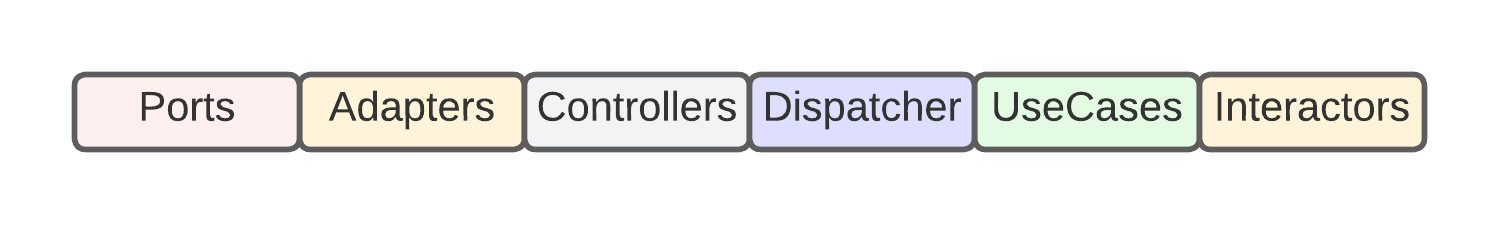
\includegraphics[width=1\textwidth]{./images/SimpliedArchitecture.png}
    \caption{Vereinfachte Darstellung}
    \label{fig:SimpliedArchitecture}
\end{figure}

Und bei einer Standalone Anwendung gibt es eine Main-Methode, die diese Struktrur erstellt.
\begin{figure}[H]
    \centering
    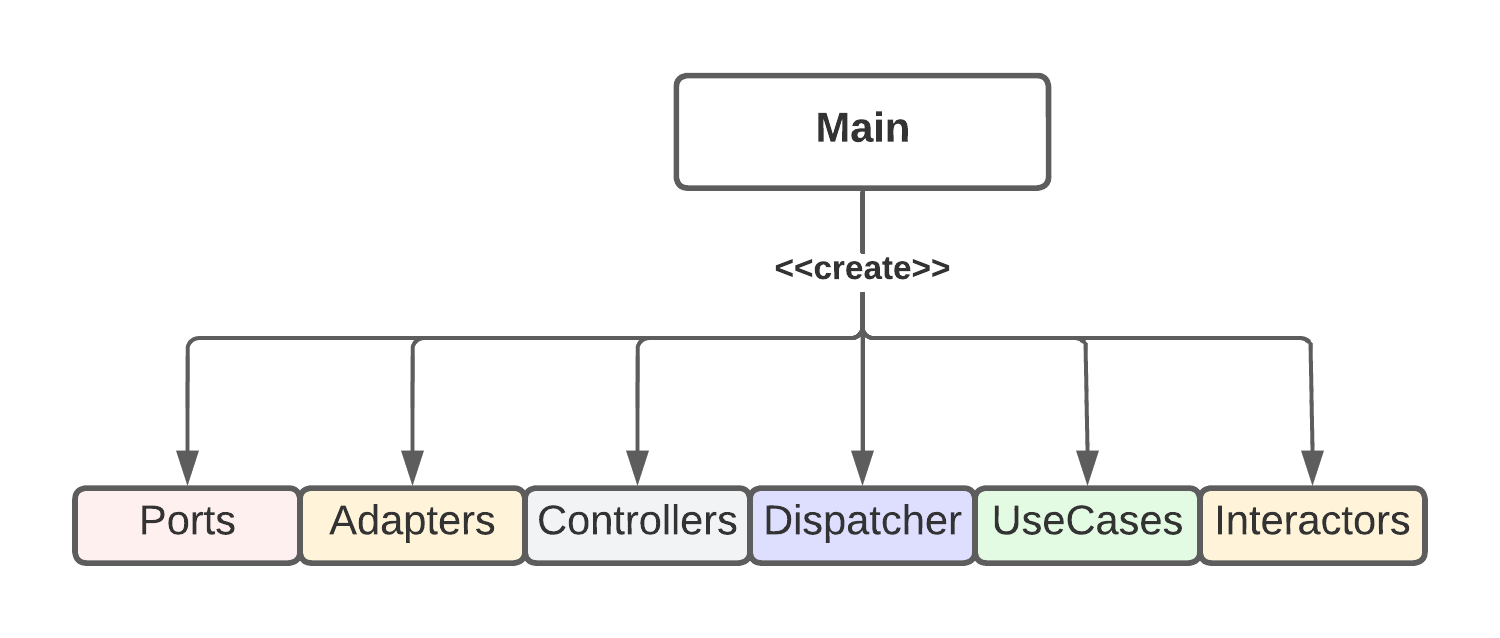
\includegraphics[width=1\textwidth]{./images/Architecture as Standalone.png}
    \caption{Vereinfachte Darstellung einer Standalone Anwendung}
    \label{fig:SimpliedArchitectureAsStandalone}
\end{figure}

Der Datenfluss lässt sich so darstellen:
\begin{figure}[H]
    \centering
    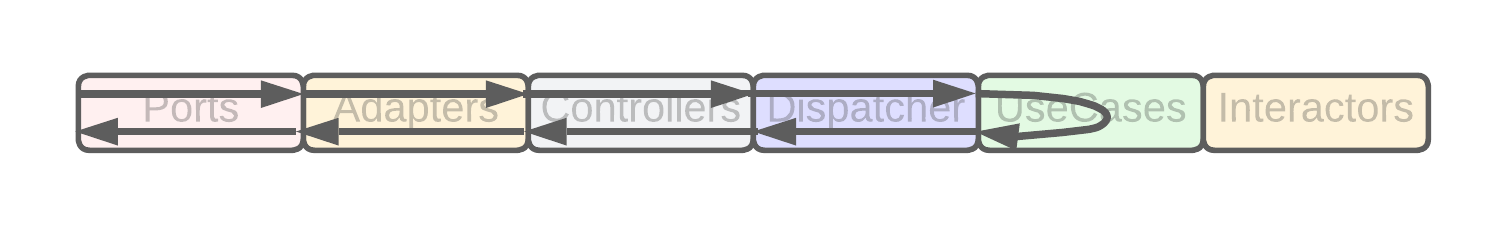
\includegraphics[width=1\textwidth]{./images/Dataflow.png}
    \caption{Vereinfachte Darstellung einer Standalone Anwendung}
    \label{fig:SimpliedArchitectureDataflow}
\end{figure}

\newpage
Wenn man es als Komponente in einer anderen Anwendung verwenden möchte, braucht die Struktur eine Fassade (Kapitel \ref{kap:gof:facade}), damit man 
auf wichtige Teile der Komponente zugreifen kann und der Rest verborgen bleibt. 
Die Fassade baut die gesamte Struktur der Komponente auf.

Eine fertige Komponente, die man in die anderen Anwendungen integrieren kann:

\begin{figure}[H]
    \centering
    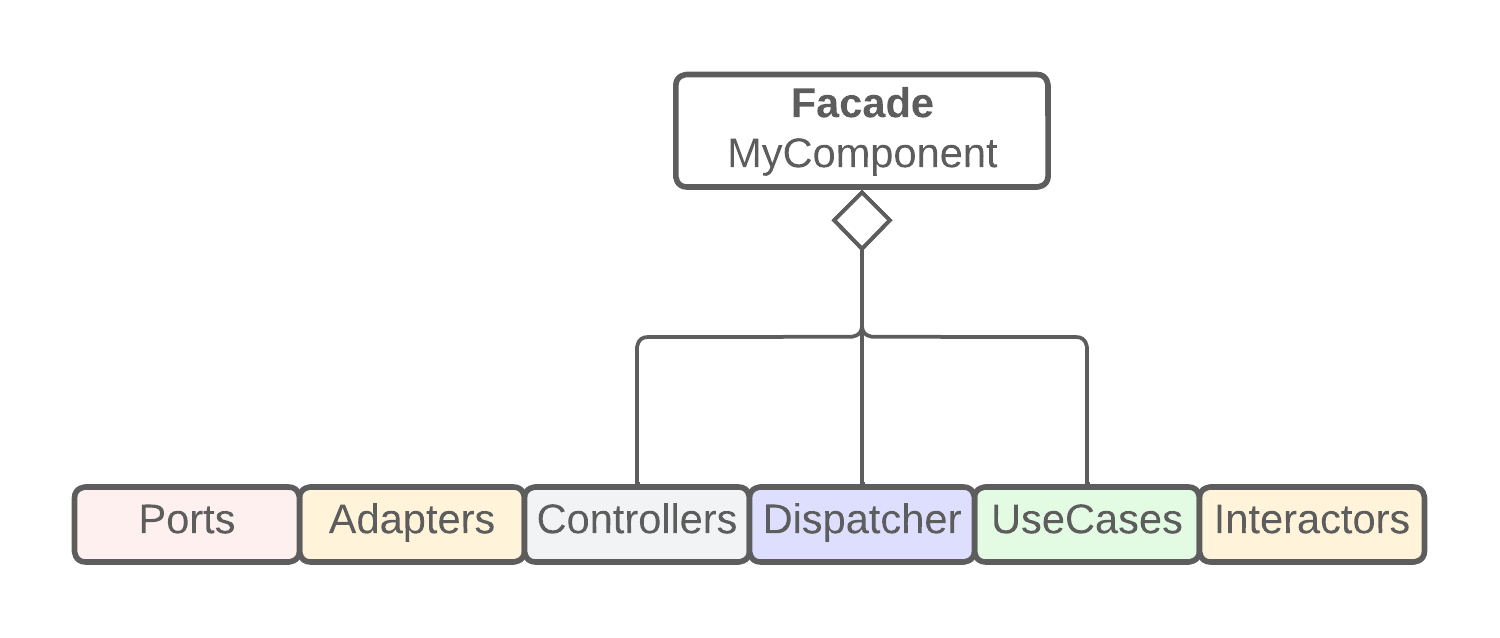
\includegraphics[width=1\textwidth]{./images/Architecture as Facade.png}
    \caption{Vereinfachte Darstellung der Architektur als Komponente}
    \label{fig:SimpliedArchitectureAsKomponent}
\end{figure}

Laut der Darstellung \ref{fig:SimpliedArchitectureAsKomponent} hat die Anwendung nur den Zugriff auf drei Teile der Komponente:
\begin{itemize}
    \item \textbf{Controllers} - um die Zustände des jeweiligen Controllers abzufragen und zu ändern.
    \item \textbf{Dispatcher} - um alle Ereignisse in der Komponente abzufangen.
    \item \textbf{UseCases} - um das Verhalten auf gewisse Ereignisse ändern zu können.
\end{itemize}

Die Komponente kann bestimmte Ereignisse selber abarbeiten und die restliche Anwendung wird darüber nicht informiert oder
das Ereignis weiterleiten, dass es von der Anwednung selbst abgearbeitet wird.
Die Komponente wird von der eigentlichen Anwendung unabhängig entwickelt, es kann passieren, dass
der Datentyp des Ereignisses von der Komponente nicht mit dem Datentyp der Anwendung übereinstimmt. 
Ein \textbf{Adapter} wäre eine mögliche Lösung für das Problem.
Das bedeutet, dass die Komponente nur von dem \textbf{Port} der jeweiligen Anwendung benutzt wird.

\newpage
Die Vereinfachte Darstellung der Anwendung mit der Komponente:
\begin{figure}[H]
    \centering
    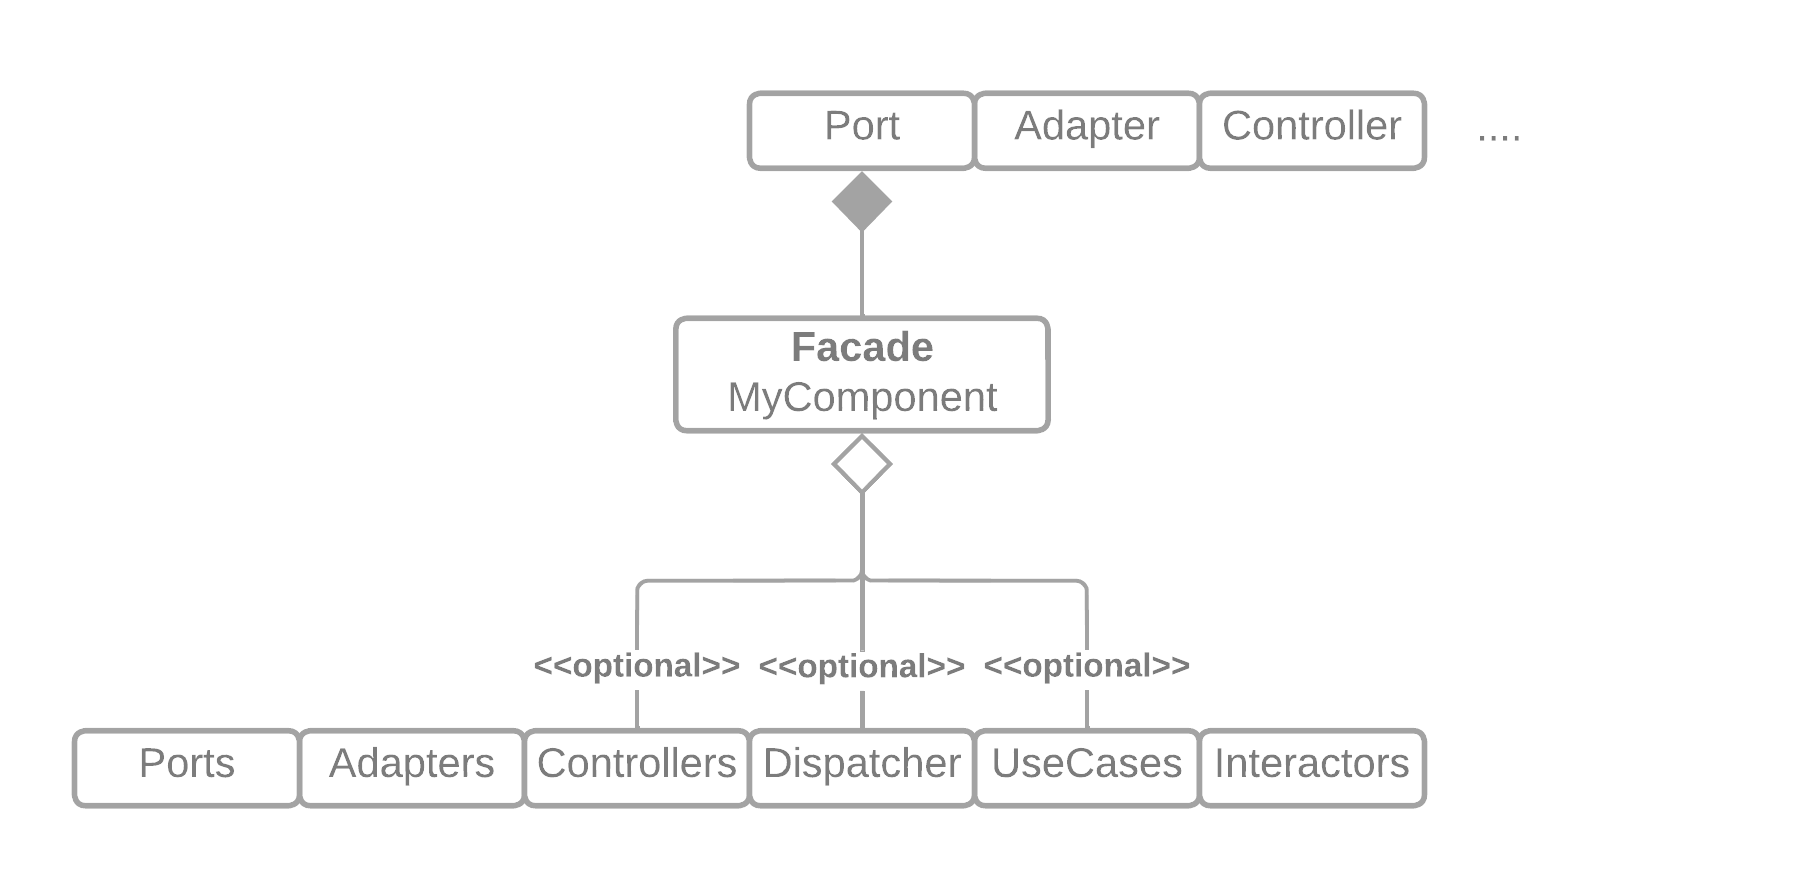
\includegraphics[width=1\textwidth]{./images/Architecture as Component.png}
    \caption{Vereinfachte Darstellung einer Standalone Anwendung mit der Komponente}
    \label{fig:SimpliedArchitectureAsStandaloneWithComponent}
\end{figure}

Der Datenfluss in der Anwendung:
\begin{figure}[H]
    \centering
    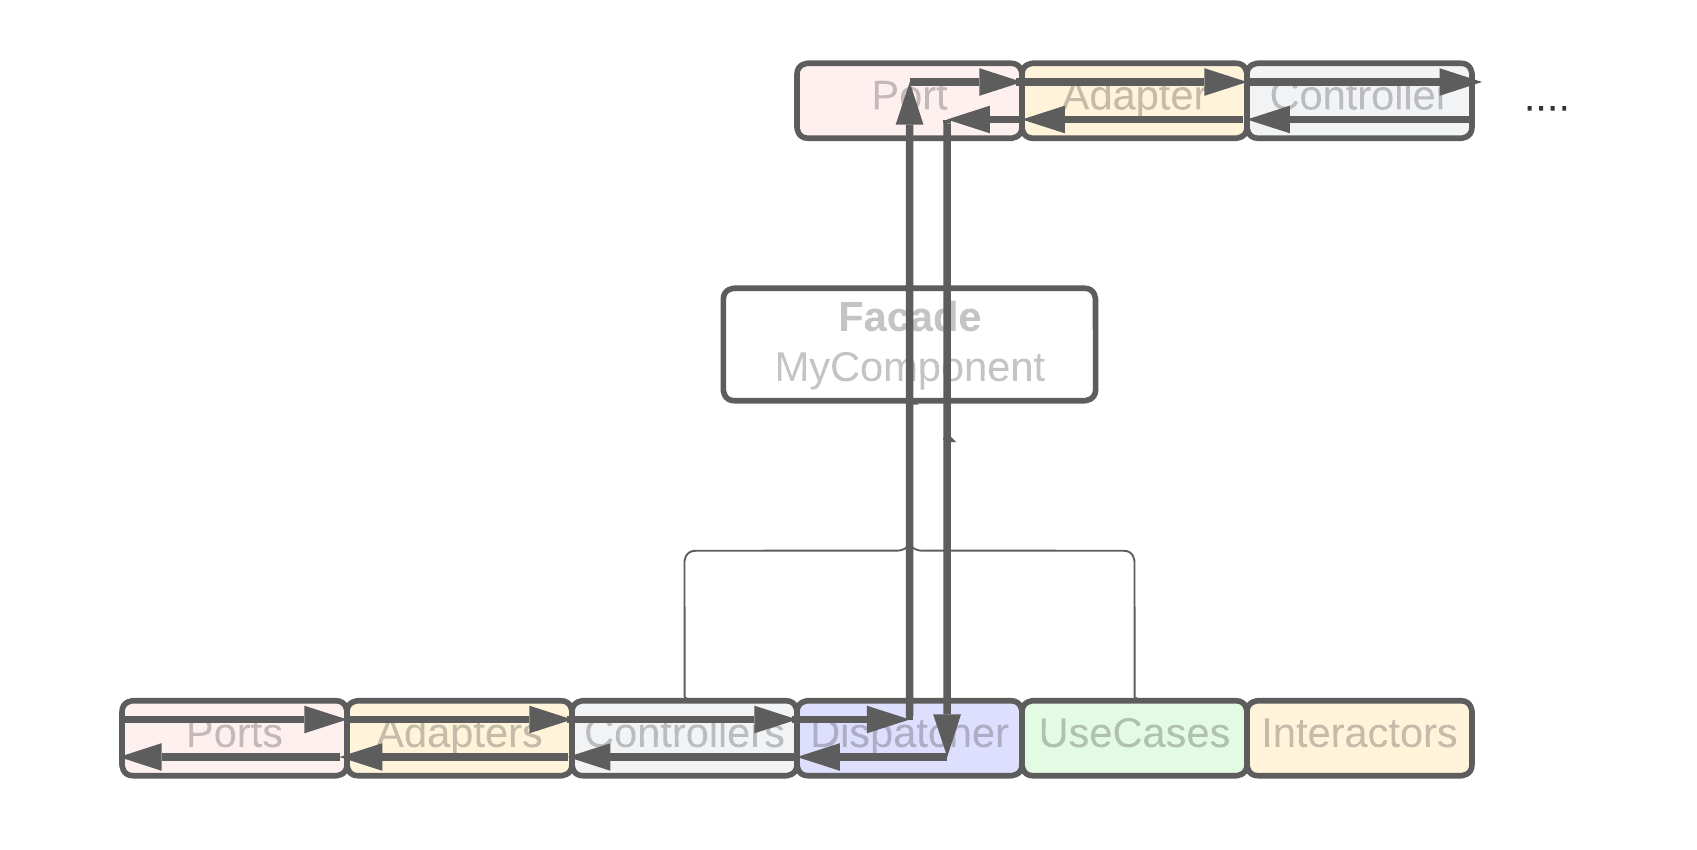
\includegraphics[width=1\textwidth]{./images/Dataflow as Component with inform.png}
    \caption{Vereinfachte Darstellung des Datenflusses in einer Anwendung mit Komponente}
    \label{fig:SimpliedDataflowWithComponent}
\end{figure}